\documentclass{beamer}
\beamertemplatenavigationsymbolsempty

\title[Asian Englishes]{Asian Englishes\\ World Englishes}
\author[Francis Bond]{Francis Bond}
\date{2024}



\usepackage{tikz}
\usepackage{graphicx}
\usepackage{fontspec}
\usepackage{xeCJK}
\setCJKmainfont{Noto Sans CJK SC}
\newfontfamily\Libertine[Mapping=tex-text]{Linux Libertine O}
\usetheme{Madrid}
\usecolortheme{crane}

\usepackage{mygb4e}
\renewcommand{\eachwordtwo}{\Libertine}
\usepackage[e,f]{mtg2e}
\usepackage{xcolor}
\renewcommand{\mtcitestyle}[1]{\textcolor{teal}{\textit{#1}}}
\newcommand{\msa}{\mtciteform}

\begin{document}

% Title Slide
\begin{frame}
    \titlepage
\end{frame}


\section{World Englishes}


% Slide 1: What Are World Englishes?
\begin{frame}{What Are World Englishes?}
\textbf{Definition:}
\begin{itemize}
    \item The global varieties of English spoken in diverse cultural, social, and linguistic contexts.
    \item Includes \textbf{Inner Circle}, \textbf{Outer Circle}, and \textbf{Expanding Circle} Englishes (Kachru, 1985).
\end{itemize}

\textbf{Importance:}
\begin{itemize}
    \item Reflects the spread of English as a global lingua franca.
    \item Highlights the adaptability and localization of English in different regions.
\end{itemize}

\textbf{Examples:}
\begin{itemize}
    \item British English, Indian English, Chinese English, Nigerian English.
\end{itemize}
\end{frame}


% Slide 4: Kachru's Three Circles
\begin{frame}{Kachru's Three Circles of English}
\centering
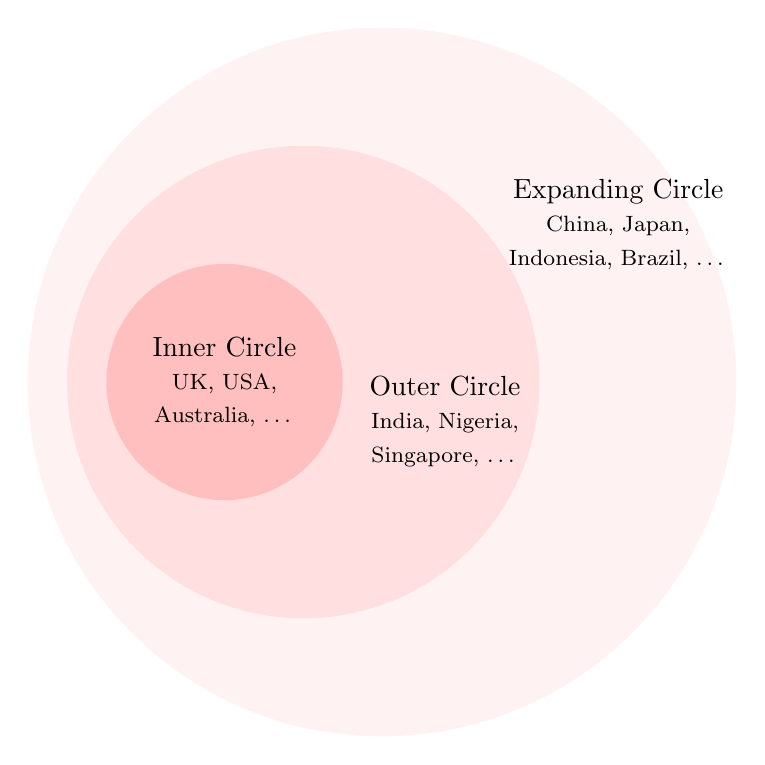
\begin{tikzpicture}
 

    % Expanding Circle
    \fill[fill=pink!20] (0,0) circle [radius=4.5];
 
    % Outer Circle
    \fill[fill=pink!50] (-1,0) circle [radius=3];
    \node[align=center] at (.8,-.5) {Outer Circle \\
      \footnotesize India, Nigeria, \\  \footnotesize Singapore, \ldots};

   % Inner Circle
  \fill[fill=pink] (-2,0) circle [radius=1.5];
  \node[align=center] at (-2,0) {Inner Circle\\
    \footnotesize UK, USA, \\  \footnotesize  Australia, \ldots};

  \node[align=center] at (3, 2) {Expanding Circle \\ \footnotesize China, Japan,  \\ \footnotesize Indonesia, Brazil, \ldots};

  \end{tikzpicture}
\end{frame}


\begin{frame}{The Inner Circle}
\textbf{Definition:}
\begin{itemize}
    \item Represents countries where English is the native language and primary means of communication.
\end{itemize}

\textbf{Examples:}
\begin{itemize}
    \item United Kingdom, United States, Australia, Canada, New Zealand.
\end{itemize}

\textbf{Key Features:}
\begin{itemize}
    \item Historical origin of English.
    \item Sets linguistic norms often viewed as "standard" English.
    \item Used as a cultural identifier.
\end{itemize}

\end{frame}

% Slide 2: Outer Circle
\begin{frame}{The Outer Circle}
\textbf{Definition:}
\begin{itemize}
    \item Countries where English serves as a second language, often used in government, education, and business.
    \item Reflects historical colonial influence.
\end{itemize}

\textbf{Examples:}
\begin{itemize}
\item India, Nigeria, Singapore, Philippines.
\item Singapore fits all characteristics of inner circle except origin, \ldots
\end{itemize}

\textbf{Key Features:}
\begin{itemize}
    \item Nativized varieties of English.
    \item High degree of multilingualism among speakers.
    \item Functional roles in administration and education.
    \item More speakers than the inner circle
\end{itemize}

\end{frame}

% Slide 3: Expanding Circle
\begin{frame}{The Expanding Circle}
\textbf{Definition:}
\begin{itemize}
    \item Countries where English is used as a foreign language.
    \item Primarily for international communication and business.
\end{itemize}

\textbf{Examples:}
\begin{itemize}
    \item China, Japan, Brazil, Russia.
\end{itemize}

\textbf{Key Features:}
\begin{itemize}
    \item Does not have a colonial legacy of English.
    \item Lacks institutionalized functions in government or education.
    \item Growing role in globalization and digital communication.
    \item Has the most speakers!
\end{itemize}

\end{frame}
\begin{frame}{English-speaking populations across various countries.}
  \begin{center}
\small
\begin{tabular}{lrrrrrrr}
  \textbf{Country} & \textbf{ Population} & \textbf{Speakers }  & \textbf{First L}  & \textbf{Other L}  \\ \hline
United States & 312,092,668 & 297,400,000 & 244,232,103 & 42,155,719 \\ 
India & 1,450,000,000 & 228,539,090 & 259,678 & 228,279,412 \\ 
Nigeria & 206,200,000 & 125,039,680 & 20,000,000 & 103,198,040  \\ 
Pakistan & 220,892,331 & 108,044,691 & 8,642 & 108,036,049  \\ 
United Kingdom & 64,000,000 & 62,912,000 & 59,072,000 & 3,840,000 \\ 
Philippines & 110,000,000 & 70,117,935 & 36,935 & 70,081,000  \\ 
Germany & 80,600,000 & 45,400,000 & 392,000 & 45,100,000  \\ 
Uganda & 44,270,000 & 19,800,000 & 0 & 19,800,000  \\ 
France & 67,500,000 & 38,643,750 & 0 & 38,643,750  \\ 
Canada & 37,138,500 & 30,480,750 & 20,193,335 & 10,287,415  \\ 
Egypt & 110,990,000 & 44,373,802 & 5,527,302 & 38,846,500  \\ 
Australia & 23,401,892 & 21,715,910 & 17,020,421 & 4,695,489  \\ 
Bangladesh & 165,323,100 & 19,838,772 & 709,873 & 16,398,158 \\ 
Poland & 38,501,000 & 18,890,000 & 103,541 & 18,786,459  \\ 
Ghana & 27,000,000 & 18,000,000 & 0 & 18,000,000  \\[1ex] 
Singapore & 4,044,200 & 3,900,000 & 1,953,348 & 1,946,652 
\end{tabular}
    
\end{center}
{\footnotesize Data from  \href{https://en.wikipedia.org/wiki/List_of_countries_by_English-speaking_population}{Wikipedia: List of countries by English-speaking population}}
\end{frame}

% Slide 1: General Debate
\begin{frame}{World Englishes: Quirk vs. Kachru}
\textbf{Quirk's Perspective (Uniformity View):}
\begin{itemize}
    \item Emphasizes a single, standardized form of English based on Inner Circle norms (e.g., UK, US).
    \item Concerns about intelligibility and global communication.
    \item Argues that legitimizing non-standard varieties risks misunderstanding.
\end{itemize}

\textbf{Kachru's Perspective (Pluralist View):}
\begin{itemize}
    \item Advocates for the legitimacy of Outer Circle varieties (e.g., Indian, Nigerian English).
    \item Emphasizes linguistic and cultural adaptation (nativization).
    \item Critiques the deficit model of "errors" and promotes ownership of English by all its users.
\end{itemize}
\end{frame}

% Slide 2: Key Themes of the Debate
\begin{frame}{Key Themes of the Debate}
\begin{itemize}
    \item \textbf{Standardization vs. Diversity:}
    \begin{itemize}
        \item Quirk: Standardization is essential for global intelligibility.
        \item Kachru: Diversity reflects the realities of English use worldwide.
    \end{itemize}
    \item \textbf{Pedagogical Implications:}
    \begin{itemize}
        \item Quirk: Teaching should adhere to Inner Circle norms.
        \item Kachru: Teaching should validate localized varieties.
    \end{itemize}
    \item \textbf{Ownership of English:}
    \begin{itemize}
        \item Quirk: English belongs to the Inner Circle.
        \item Kachru: English is the global property of all its users.
    \end{itemize}
\end{itemize}
\end{frame}

% Slide 3: Kachru's Four False Assumptions
\begin{frame}{Kachru's Critique: Four False Assumptions}
\textbf{1. The Homogeneity Assumption:}
\begin{itemize}
    \item Assumes a single, homogeneous standard English.
    \item Counterpoint: Inner Circle varieties themselves exhibit variation.
\end{itemize}

\textbf{2. The Deficit Model of Non-Native Varieties:}
\begin{itemize}
    \item Views Outer Circle Englishes as "deviant."
    \item Counterpoint: Outer Circle varieties are contextually legitimate adaptations.
\end{itemize}

\textbf{3. The Pedagogical Purity Assumption:}
\begin{itemize}
    \item Insists on teaching Inner Circle norms exclusively.
    \item Counterpoint: Teaching should reflect local linguistic realities.
\end{itemize}

\textbf{4. The Intelligibility Assumption:}
\begin{itemize}
    \item Claims Inner Circle norms ensure mutual intelligibility.
    \item Counterpoint: Intelligibility is context-dependent and mutual.
\end{itemize}
\end{frame}


% Slide B4: The Legitimate and Illegitimate Offspring of English
\begin{frame}{B4: The Legitimate and Illegitimate Offspring of English}
\textbf{The Naming of the New Englishes (Mufwene, 1997):}
\begin{itemize}
    \item Criticism of Western linguists’ terminology.
    \item Based on mistaken belief:
    \begin{itemize}
        \item "Mother language" gives birth to "daughter language" without contact.
    \end{itemize}
    \item Language contact also a feature of "legitimate" Englishes.
\end{itemize}
\end{frame}

% Slide B4: Innovation – Deviation – Mistake
\begin{frame}{B4: Innovation – Deviation – Mistake (Kachru, 1992)}
\textbf{Key Distinctions:}
\begin{itemize}
    \item \textbf{Innovation:} Creativity in language use; often denied to Outer and Expanding Circle speakers.
    \item \textbf{Deviation:} Comparison with another variety; implies departure from a norm.
    \item \textbf{Mistake (or error):} Related to acquisitional deficiency.
\end{itemize}
\end{frame}

% Slide B5: Standards Across Space
\begin{frame}{B5: Standards Across Space}
\textbf{Three "Standard" Englishes:}
\begin{itemize}
    \item Britain, North America, Australia.
    \item Similarities and differences:
    \begin{itemize}
        \item Across the three standards.
        \item Across varieties within each region (e.g., UK, US).
    \end{itemize}
\end{itemize}
\end{frame}

% Slide B5: Vocabulary Divergences
\begin{frame}{B5: Vocabulary Divergences}
\textbf{Vocabulary: The Most Noticeable Divergence (NAmE vs. BrE):}
\begin{itemize}
    \item Early settlers introduced:
    \begin{itemize}
        \item \textbf{Extended meanings:} e.g., corn, robin.
        \item \textbf{New words:} e.g., buttle.
        \item \textbf{Borrowings:} e.g., moccasin, squash, toboggan.
    \end{itemize}
    \item Since US independence:
    \begin{itemize}
        \item Technological terms: e.g., windshield vs. windscreen.
    \end{itemize}
\end{itemize}
\end{frame}

% Slide B5: Categories of Lexical Differences
\begin{frame}{Categories of Lexical Differences}
\textbf{Trudgill and Hannah (2002):}
\begin{itemize}
    \item Same word, different meaning.
    \item Same word, additional meaning in one variety.
    \item Same word, difference in style, connotation, or frequency.
    \item Same concept or item, different word.
\end{itemize}
\end{frame}

% Slide B5: Australian English
\begin{frame}{Australian English}
\textbf{Key Features:}
\begin{itemize}
    \item Borrowings from Aboriginal languages: e.g., \eng{kangaroo, boomerang}.
    \item Unique slang words and phrases.
    \item Common use of abbreviations and clippings.
      \\ \eng[bbq]{barbie}, \eng[university]{uni}, \eng[sandwich]{sammy}, \eng[relative]{relly}, \eng[U-turn]{chuck a uey}
      \\ \eng[person with white hair]{Snowy}, \eng[red-head]{Bluey}, \eng[me]{Bondie}
\end{itemize}
\end{frame}

% Slide B5: Grammar Differences
\begin{frame}{Grammar Differences}
\textbf{USEng vs. EngEng (Trudgill and Hannah, 2002):}
\begin{itemize}
    \item Verbs: morphology, auxiliaries.
    \item Nouns: endings, use of verbs as nouns.
    \item Adjectives and adverbs.
    \item Prepositions.
\end{itemize}
\end{frame}

% Slide B6: Native and Non-Native Speakers
\begin{frame}{Native and Non-Native Speakers of English}
\textbf{Criticisms of NS/NNS Terms:}
\begin{itemize}
    \item Assumes monolingualism is the norm.
    \item Overemphasizes order of acquisition.
    \item Reinforces Anglo speakers as reference points.
    \item Implies unidirectional power relationships.
    \item Encourages simplistic views of "errors."
\end{itemize}
\end{frame}

% Slide B6: Alternatives to NS/NNS
\begin{frame}{Alternatives to NS/NNS Distinction}
\textbf{Rampton (1990): "Experts" $\rightarrow$ Expertise}
\begin{itemize}
    \item Advantages:
    \begin{itemize}
        \item Learned, not innate.
        \item Relative, partial, and contestable.
    \end{itemize}
    \item Disadvantages:
    \begin{itemize}
        \item "Non-expert" implies value judgment.
    \end{itemize}
\end{itemize}

\textbf{Jenkins (1996, 2000): MES, BES, NBES}
\begin{itemize}
    \item MES: Monolingual English Speaker.
    \item BES: Bilingual English Speaker.
    \item NBES: Non-Bilingual English Speaker.
\end{itemize}
\end{frame}

% Slide B7: Codification of Asian Englishes
\begin{frame}{En Route to New Standard Englishes}
\textbf{Codification of Asian Englishes:}
\begin{itemize}
    \item Importance:
    \begin{itemize}
        \item Acceptance, prestige, classroom model.
    \end{itemize}
    \item Obstacles:
    \begin{itemize}
        \item Indigenized varieties seen as "interlanguages."
        \item SLA perspective emphasizes NS-like competence.
        \item Motivation for acquisition is integrative (admiration for NS culture).
    \end{itemize}
\end{itemize}
\end{frame}



% Slide 3: Characteristics of Asian Englishes
\begin{frame}{Characteristics of Asian Englishes}
\textbf{Distinct Features:}
\begin{itemize}
    \item \textbf{Phonology:} Unique accents and stress patterns (e.g., Indian English retroflex sounds).
    \item \textbf{Syntax:} Influence of local languages (e.g., omission of articles in Singapore English).
    \item \textbf{Lexicon:} Borrowings and cultural terms (e.g., "chop" in Malaysian English for "stamp").
\end{itemize}

\textbf{Examples:}
\begin{itemize}
    \item Indian English: Distinct grammar (e.g., "prepone" for schedule advancement).
    \item Filipino English: Code-switching with Tagalog.
    \item Singapore English: "Singlish" with local idioms and particles.
\end{itemize}
\end{frame}

\section{Indian English}

\begin{frame}
\frametitle{What is Indian English?}
\begin{itemize}
    \item Indian English refers to the variety of English spoken in India.
    \item It is influenced by India's multilingual environment and local languages.
    \item Features unique vocabulary, pronunciation, grammar, and idiomatic expressions.
    \item Recognized as one of the most widespread second languages in India.
\end{itemize}
\end{frame}

\begin{frame}
\frametitle{Key Features of Indian English}
\begin{itemize}
    \item \textbf{Pronunciation:}
    \begin{itemize}
        \item Rhotic: Pronouncing /r/ in words like "car" and "farm."
        \item Flattened vowels: "bat" may sound like "baet."
    \end{itemize}
    \item \textbf{Vocabulary:}
    \begin{itemize}
        \item Unique words like "prepone" (to reschedule earlier) and "godown" (warehouse).
    \end{itemize}
    \item \textbf{Grammar:}
    \begin{itemize}
        \item Use of the progressive tense: "He is knowing the answer."
    \end{itemize}
\end{itemize}
\end{frame}

\begin{frame}
\frametitle{Unique Vocabulary in Indian English}
\begin{itemize}
    \item \textbf{Borrowed words:}
    \begin{itemize}
        \item Bungalow (from Hindi: "bangla")
        \item Jungle (from Hindi: "jangal")
    \end{itemize}
    \item \textbf{Hybrid expressions:}
    \begin{itemize}
        \item "Pass out" (to graduate)
        \item "Out of station" (not in town)
    \end{itemize}
    \item \textbf{Local adaptations:}
    \begin{itemize}
        \item "Hill station" (mountain resort)
        \item "Timepass" (leisure activity)
    \end{itemize}
\end{itemize}
\end{frame}

\begin{frame}
\frametitle{Examples of Indian English Sentences}
\begin{itemize}
    \item "Can you prepone the meeting to tomorrow?"
    \item "I passed out of college in 2020."
    \item "He is having a doubt in mathematics."
    \item "She went to the market to buy vegetables only."
    \item "Let us go for a walk in the evening, no?"
\end{itemize}
\end{frame}

\begin{frame}
\frametitle{Cultural and Linguistic Significance}
\begin{itemize}
    \item Indian English reflects the diversity of India's languages and cultures.
    \item It bridges communication gaps in a multilingual society.
    \item Used in government, education, business, and media.
    \item Contributes to the global spread of English with a distinct identity.
\end{itemize}
\end{frame}


\section{Singlish (Manglish)}


\begin{frame}
\frametitle{What is Singlish?}
\begin{itemize}
    \item Singlish is the colloquial form of English spoken in Singapore.
    \item It combines English with elements from Malay, Tamil, Hokkien, Cantonese, and other languages.
    \item Singlish is informal and often spoken in casual settings.
    \item Although not officially endorsed, it is a key part of Singaporean identity.
\end{itemize}
\end{frame}

\begin{frame}
\frametitle{Key Features of Singlish}
\begin{itemize}
    \item \textbf{Vocabulary:}
    \begin{itemize}
        \item Borrowed words like "lah" (emphasis) and "kiasu" (fear of missing out).
    \end{itemize}
    \item \textbf{Grammar:}
    \begin{itemize}
        \item Simplified grammar: "I go there yesterday" (instead of "I went there yesterday").
    \end{itemize}
    \item \textbf{Particle usage:}
    \begin{itemize}
        \item "Lah," "lor," "meh," and "ah" add tone or meaning to sentences.
    \end{itemize}
\end{itemize}
\end{frame}

\begin{frame}
\frametitle{Examples of Singlish Vocabulary}
\begin{itemize}
    \item \textbf{Common words and phrases:}
    \begin{itemize}
        \item \textbf{Lah:} "Don't worry lah!" (adds emphasis or assurance)
        \item \textbf{Kiasu:} "He is so kiasu." (fear of missing out)
        \item \textbf{Shiok:} "This food is so shiok!" (delicious or enjoyable)
        \item \textbf{Blur:} "Why are you so blur?" (confused or clueless)
    \end{itemize}
    \item \textbf{Borrowed terms:}
    \begin{itemize}
        \item \textbf{Paiseh:} "So paiseh to ask!" (embarrassed)
        \item \textbf{Ang moh:} "The ang moh loves laksa." (Caucasian)
    \end{itemize}
\end{itemize}
\end{frame}

\begin{frame}
\frametitle{Singlish Grammar and Syntax}
\begin{itemize}
    \item \textbf{Sentence simplification:}
    \begin{itemize}
        \item "He go already." (He has already gone.)
    \end{itemize}
    \item \textbf{Tag particles:}
    \begin{itemize}
        \item "You want coffee, ah?" (adds a questioning tone)
        \item "Very expensive, leh." (adds emphasis)
    \end{itemize}
    \item \textbf{Omission of articles:}
    \begin{itemize}
        \item "I go market." (I am going to the market.)
    \end{itemize}
\end{itemize}
\end{frame}

\begin{frame}
\frametitle{Cultural and Linguistic Significance}
\begin{itemize}
    \item Singlish reflects Singapore’s multicultural heritage.
    \item It fosters a sense of local identity and camaraderie.
    \item Often used in media, humor, and casual conversations.
    \item Despite government efforts to promote Standard English, Singlish remains a vibrant and unique aspect of Singaporean culture.
\end{itemize}
\end{frame}


\section{Hong Kong English}



\begin{frame}
\frametitle{What is Hong Kong English?}
\begin{itemize}
    \item Hong Kong English is the variety of English influenced by Cantonese, the primary language spoken in Hong Kong.
    \item Developed due to British colonial rule (1842–1997) and remains significant in education, business, and law.
    \item Reflects a blend of British English, local linguistic features, and Cantonese cultural influence.
\end{itemize}
\end{frame}

\begin{frame}
\frametitle{Key Features of Hong Kong English}
\begin{itemize}
    \item \textbf{Pronunciation:}
    \begin{itemize}
        \item Influence of Cantonese tones on stress patterns.
        \item /r/ and /l/ sounds may overlap (e.g., "rice" pronounced as "lice").
    \end{itemize}
    \item \textbf{Grammar:}
    \begin{itemize}
        \item Omission of articles and prepositions: "I go market" (I am going to the market).
    \end{itemize}
    \item \textbf{Vocabulary:}
    \begin{itemize}
        \item Loanwords from Cantonese: "yum cha" (drink tea) and "char siu" (roast pork).
    \end{itemize}
\end{itemize}
\end{frame}

\begin{frame}
\frametitle{Examples of Hong Kong English Vocabulary}
\begin{itemize}
    \item \textbf{Loanwords from Cantonese:}
    \begin{itemize}
        \item \textbf{Dai pai dong:} Open-air food stalls.
        \item \textbf{Si fu:} Master or skilled worker.
        \item \textbf{Cha chaan teng:} Hong Kong-style cafes.
    \end{itemize}
    \item \textbf{Hybrid expressions:}
    \begin{itemize}
        \item \textbf{Add oil:} An encouragement or cheer, meaning "keep going" or "good luck."
        \item \textbf{Long time no see:} A literal translation of the Cantonese phrase "好耐冇見" (hou noi mou gin).
    \end{itemize}
\end{itemize}
\end{frame}

\begin{frame}
\frametitle{Common Features of Sentences in Hong Kong English}
\begin{itemize}
    \item \textbf{Direct translations from Cantonese:}
    \begin{itemize}
        \item "He very smart, la." (He is very smart, you know.)
    \end{itemize}
    \item \textbf{Omission of grammatical elements:}
    \begin{itemize}
        \item "I no understand." (I do not understand.)
    \end{itemize}
    \item \textbf{Unique phrases:}
    \begin{itemize}
        \item "I go yum cha with family tomorrow." (I am going to have dim sum with my family tomorrow.)
    \end{itemize}
\end{itemize}
\end{frame}

\begin{frame}
\frametitle{Cultural and Linguistic Significance}
\begin{itemize}
    \item Hong Kong English reflects the region’s colonial past and its Cantonese-speaking majority.
    \item It plays a key role in education, government, and international business.
    \item Highlights the blending of British and Chinese cultures in Hong Kong.
    \item Despite its informal and localized nature, it remains an essential aspect of Hong Kong’s identity and communication in multilingual settings.
\end{itemize}
\end{frame}


\section{Japanese English (Japlish/Engrish)}



\begin{frame}
\frametitle{What is Japanese English?}
\begin{itemize}
    \item Japanese English refers to the variety of English influenced by the Japanese language.
    \item It often features adaptations of English words and phrases to fit Japanese phonetics and culture.
    \item Developed due to English education, international business, and cultural exchange.
    \item Known for unique loanwords, katakana usage, and creative expressions.
\end{itemize}
\end{frame}

\begin{frame}
\frametitle{Key Features of Japanese English}
\begin{itemize}
    \item \textbf{Phonetic adjustments:}
    \begin{itemize}
        \item Inserting vowels: "table" becomes "te-bu-ru."
        \item No distinction between /l/ and /r/: "light" and "right" sound similar.
    \end{itemize}
    \item \textbf{Vocabulary:}
    \begin{itemize}
        \item Loanwords adapted to Japanese: "salaryman" (businessman), "OL" (office lady).
    \end{itemize}
    \item \textbf{Grammar:}
    \begin{itemize}
        \item Direct translations from Japanese syntax.
    \end{itemize}
\end{itemize}
\end{frame}

\begin{frame}
\frametitle{Examples of Japanglish Vocabulary}
\begin{itemize}
    \item \textbf{Adapted loanwords:}
    \begin{itemize}
        \item \textbf{Salaryman:} Office worker.
        \item \textbf{Hand phone:} Mobile phone (from "handy phone").
        \item \textbf{Viking:} Buffet (originating from "smorgasbord").
    \end{itemize}
    \item \textbf{Hybrid expressions:}
    \begin{itemize}
        \item \textbf{My pace:} Going at one's own speed.
        \item \textbf{Skinship:} Physical closeness or bonding.
    \end{itemize}
    \item \textbf{Creative coinages:}
    \begin{itemize}
        \item \textbf{Power harassment:} Workplace bullying.
        \item \textbf{Conveni:} Convenience store.
    \end{itemize}
\end{itemize}
\end{frame}

\begin{frame}
\frametitle{Common Sentence Structures in Japanese English}
\begin{itemize}
    \item \textbf{Direct translations from Japanese:}
    \begin{itemize}
        \item "Please enjoy!" (Enjoy yourself.)
        \item "I will do my best." (A translation of "ganbarimasu.")
    \end{itemize}
    \item \textbf{Simplified grammar:}
    \begin{itemize}
        \item "He go to school every day." (Missing "s" in "goes.")
    \end{itemize}
    \item \textbf{Mixing Japanese and English:}
    \begin{itemize}
        \item "Let’s go to izakaya for nomikai." ("Let’s go to a pub for drinks.")
    \end{itemize}
\end{itemize}
\end{frame}

\begin{frame}
\frametitle{Cultural and Linguistic Significance}
\begin{itemize}
    \item Japanese English showcases the cultural blending of Japan and the English-speaking world.
    \item Reflects creative adaptations to fit Japanese language structure and social norms.
    \item Plays an important role in education, tourism, and advertising in Japan.
    \item Despite challenges with pronunciation and syntax, it has become a unique and recognizable form of English globally.
\end{itemize}
\end{frame}









% Slide 4: Challenges and Opportunities
\begin{frame}{Challenges and Opportunities for Asian Englishes}
\textbf{Challenges:}
\begin{itemize}
    \item Perceived legitimacy: Often compared to Inner Circle varieties.
    \item Codification: Lack of formal standards for some varieties.
    \item Pedagogy: Balancing local and global intelligibility.
\end{itemize}

\textbf{Opportunities:}
\begin{itemize}
    \item Reflects local identity and culture.
    \item Encourages creativity and linguistic innovation.
    \item Promotes multilingualism and cross-cultural communication.
\end{itemize}
\end{frame}

% Slide 5: The Future of Asian Englishes
\begin{frame}{The Future of Asian Englishes}
\textbf{Trends:}
\begin{itemize}
    \item Increasing prestige and global recognition.
    \item Growth of English as a second language in Asia.
    \item Integration into educational systems and digital platforms.
\end{itemize}

\textbf{Key Questions:}
\begin{itemize}
    \item How will globalization shape Asian Englishes?
    \item Will codification lead to the emergence of new standards?
    \item How can we balance intelligibility and diversity?
\end{itemize}

\textbf{Conclusion:}
\begin{itemize}
    \item Asian Englishes showcase the dynamic evolution of the language.
    \item They are key to understanding the future of global English.
\end{itemize}
\end{frame}



% References Slide
\begin{frame}{References}
\begin{itemize}
    \item Kachru, B. B. (1985). Standards, codification and sociolinguistic realism: The English language in the Outer Circle. In \textit{English in the World: Teaching and Learning the Language and Literatures}, edited by R. Quirk and H. Widdowson, Cambridge University Press, pp. 11–30.
    \item Quirk, R. (1985). The English language in a global context. In \textit{English in the World: Teaching and Learning the Language and Literatures}, edited by R. Quirk and H. Widdowson, Cambridge University Press, pp. 1–10.
\end{itemize}
\end{frame}

\end{document}


%%% Local Variables: 
%%% coding: utf-8
%%% mode: latex
%%% TeX-PDF-mode: t
%%% TeX-engine: xetex
%%% End: 
